\section{Anyagi tulajdonságok}

\emph{Hőtágulás: lineáris és térfogati; Különleges viselkedésű anyagok; Kompresszibilitás; Feszültségi együttható; Hármasszabály; Összefüggés az anyagi paraméterek között; Ideális gáz anyagi tulajdonságai.}

Kísérleti tapasztalat, hogy ha fémrudat melegítünk, akkor annak a hossza megnő. Sőt általánosan is igaz, hogy hőmérsékletváltozás hatására a testek hossza, térfogata megváltozik. Sok esetben a hőmérséklet és a hossz között lineáris kapcsolat áll fent, ahol az \aref{fig:termo_2_1}. ábrán is látható:
\begin{align}
    l = l_0(1+\alpha' T),
\end{align}
ahol $\alpha'$ a \emph{lineáris hőtágulási együttható}. Némely esetben azonban a hossz és  a hőmérséklet között teljesen bonyolult kapcsolat is lehet\footnote{\,Gondoljunk csak például a vízre, melynek a sűrűsége 4$^\circ$C körül a legnagyobb, ezért szoktak elfagyni a vízvezetékek, ha nem zárják el azt télre. Másik érdekes anyag a gumi. Kipróbálhatjuk, hogy befőttesgumit berakunk a fagyasztóba. Azt fogjuk tapasztalni, hogy a fagyasztóból kivett befőttesgumi összemegy.}, ekkor az $l(T)$ görbe érintőjét tudjuk csak meghatározni, ahogy az \aref{fig:termo_2_2}. ábrán is látható.
\begin{figure}[!h]
    \centering
    \begin{subfigure}[t]{0.45\textwidth}
            \centering
            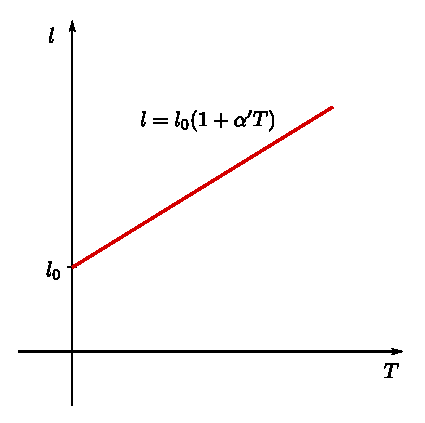
\includegraphics[width=\textwidth]{termo_2/termo_2_1}
            \newsubcap{Hőtágulás lineáris hőtágulási együtthatóval.}
            \label{fig:termo_2_1}
    \end{subfigure}\hfill
    \begin{subfigure}[t]{0.45\textwidth}
            \centering
            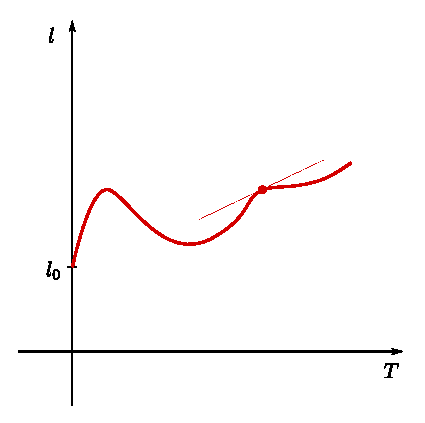
\includegraphics[width=\textwidth]{termo_2/termo_2_2}
            \newsubcap{Hőtágulás bonyolult alakú hőtágulási együtthatóval, amikor csak az adott hőmérséklethez tartozó érintőből határozható meg a hőtágulási együttható.}
            \label{fig:termo_2_2}
    \end{subfigure}
    \end{figure}
Az állandó nyomáson vett lineáris hőtágulási együttható általános esetben definíció szerint:
\begin{align}
    \alpha = \rec l \pd{l}{T}\bigg|_\pres,
\end{align}
ami tehát megadja, hogy állandó nyomáson a test hőmérsékletét változtatva mennyivel változik meg annak a hossza. Az $1/l$ azért van beledefiniálva, hogy a test hosszától független, csak az anyagi minőségtől függő mennyiséget kapjunk. A definíció szerint $[\alpha]~{=}~\frac 1K$, értéke pedig szilárd testekre $\alpha_{\tn{szilárd}}~{\sim}~10^{-5} \frac 1K$, míg folyadékokra $\alpha_{\tn{folyadék}}~{\sim}~10^{-4} \frac 1K$. Érdemes észrevenni, hogy általában $\alpha\neq\alpha'$, hiszen a $\alpha$ esetében mindig az aktuális hosszal osztunk le:
\begin{align}
    l(T) = l_0(1+\alpha' T)\Rightarrow \Delta l = l_0\alpha' T \Rightarrow \alpha = \rec l \pd{l}{T}\bigg|_\pres = \rec{l_0(1+\alpha' T)}l_0\alpha' = \frac{\alpha'}{1+\alpha' T}.
\end{align}
Ha a hőtágulási együttható negatív az azt jelenti, hogy az anyag a hőmérséklet növelésével összemegy, ilyen például a víz 0$^\circ$C és 4$^\circ$C között, a gumiszál, a damil, a vasdrót 1000$^\circ$C-on illetve a szilícium 18K-120K között.

Hőmérsékletváltozás hatására nem csak az anyagok hossza, hanem a térfogata is megváltozik. Egy $l$ oldalú kocka térfogatváltozása:
\begin{align}
\begin{split}
    V &= l^3 = \big(l_0(1+\alpha' T) \big)^3 = \underbrace{l_0^3}_{=V_0}(1+3\alpha' T +3{\alpha'}^2 T^2 + {\alpha'}^3 T^3) =\\
    &=V_0(1+\underbrace{3\alpha'}_{\beta'} T) + \mathcal O({\alpha'}^2) \approx V_0(1+\beta' T),
\end{split}
\end{align}
ahol felhasználtuk hogy $\alpha'$ másodrendűen kicsi\footnote{\,Ezt jelöltük a ,,nagy ordó'' szimbólummal, $\mathcal O$, az argumentumában szereplő mennyiségekkel, illetve azok magasabb rendű hatványai elhanyagolhatóak.}, így csak a lineáris rendig mentünk el. Bevezettük a $\beta' = 3\alpha'$ \emph{térfogati hőtágulási együtthatót} is, mely általános esetben állandó nyomáson definíció szerint:
\begin{align}
    \beta = \rec V \pd{V}{T}\bigg|_\pres,
\end{align}
ahol az $1/V$ újfent azért kellett, hogy csak az anyagi minőségtől függő állandót kapjunk, továbbá $\beta\neq\beta'$. Állandó nyomáson vett lineáris térfogati hőtágulási együtthatóra láthatunk néhány példát \aref{fig:termo_2_3}. ábrán. Ideális gáz esetében:
\begin{align}
    V = \frac{nRT}{\pres} \follows \pd{V}{T}\bigg|_\pres = \frac{nR}{\pres} \follows \beta_{\tn{id.g.}} = \frac{nR}{\pres V}=\rec T,
\end{align}
ami $T = 273{,}16$K esetén megegyezik az ideális gáz esetén bevezetett $\beta'$-vel ($\beta' = \rec{273{,}16K}$, $\beta=\beta'(T{=}273{,}16K$)). A hőmérsékletet mindenhol K-ben értjük. Láthatjuk tehát, hogy az ideális gáznak lineáris a hőtágulása.

A folytonos közegek mechanikájának tárgyalása során is találkoztunk már a \emph{kompresszibilitás} fogalmával, ami állandó hőmérsékleten definíció szerint:
\begin{align}
    \kappa = -\rec V \pd{V}{\pres}\bigg|_T,
\end{align}
ahol a negatív előjel azért szerepel a definícióban, mert a derivált minden esetben negatív kell legyen, hiszen különben a rendszer instabil lenne (külső nyomás hatására kitágulna). \Aref{fig:termo_2_4}. ábrán látható néhány példa állandó hőmérsékleten vett kompresszibilitásra, ha az összefüggés lineáris. 
\begin{figure}[!h]
    \centering
    \begin{subfigure}[b]{0.48\textwidth}
            \centering
            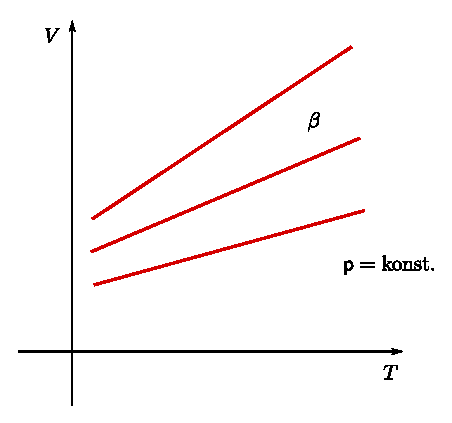
\includegraphics[width=\textwidth]{termo_2/termo_2_3}
            \newsubcap{Térfogati hőtágulás lineáris hőtágulási együtthatóval.}
            \label{fig:termo_2_3}
    \end{subfigure}\hfill
    \begin{subfigure}[b]{0.45\textwidth}
            \centering
            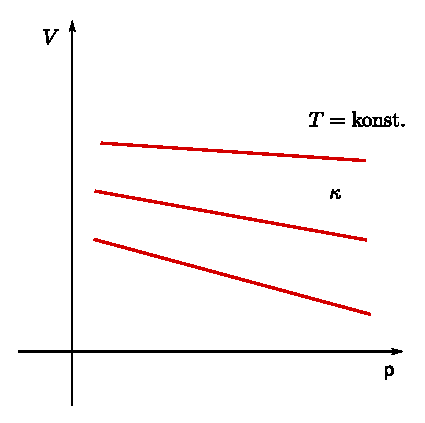
\includegraphics[width=\textwidth]{termo_2/termo_2_4}
            \newsubcap{Izoterm kompresszibilitás lineáris esetben.}
            \label{fig:termo_2_4}
    \end{subfigure}
    \end{figure}
Ideális gáz esetén:
\begin{align}
    V = \frac{nRT}{\pres} \follows \kappa_{\tn{id.g.}} = -\rec V \pd{V}{\pres}\bigg|_T = -\rec V \z{-\frac{nRT}{\pres^2}}= \rec \pres.
\end{align}
Definiálhatjuk még a \emph{feszültségi együtthatót} is állandó térfogaton a következőképp:
\begin{align}
    \gamma = \rec \pres \pd{\pres}{T}\bigg|_V,
\end{align}
mely ideális gázra:
\begin{align}
    \gamma_{\tn{id.g.}} = \rec \pres\frac{nR}{V} = \rec T.
\end{align}
A feszültségi együttható azt fejezi ki, hogy ha állandó térfogaton melegítünk egy rudat, majd lehűtjük, akkor benne feszültség keletkezik\footnote{\,Érdemes utánanézni a bolognai üvegcseppnek.}.
Mivel $\beta$, $\kappa$ és $\gamma$ definíciói meglehetősen hasonlóak, gondolhatjuk, hogy valamilyen kapcsolat áll fent ezen mérhető mennyiségek között, nem függetlenek egymástól. Induljunk ki abból, hogy az állapotegyenlet egy $f(\pres,V,T)=0$ függvény, ami egy 3d-s felületet határoz meg, lásd \aref{fig:termo_2_5}. ábrán. Ideális gáz esetében ez az összefüggés ugye $\pres V-nRT=0$. Ideiglenesen bevezetjük az alábbi jelöléseket:
\begin{align}
    \pres = \mathsf P(v,t),\quad v=V(\pres,t),\quad t=T(\pres,v).
\end{align}
Itt $\mathsf P$,$V$ és $T$ jelöli a függvényeket, $\pres$,$v$ és $t$ pedig a függvényérték. Számítsuk ki az alábbi deriváltat:
\begin{align}\label{eq:harmas_1}
    \pd{}{v}v = \pd{}{v}V(\mathsf P(v,t),t)\follows 1 = \pd V\pres\bigg|_t\cdot \pd{\mathsf P}{v}\bigg|_t.
\end{align}
Deriváljunk most $t$ szerint:
\begin{align}\label{eq:harmas_2}
    \pd{}{t}v = \pd{}{t}V(\mathsf P(v,t),t) \Rightarrow 0 = \pd{V}{\pres}\bigg|_t\cdot \pd{\mathsf P}{t}\bigg|_v+\pd{V}{t}\bigg|_\pres \Rightarrow \pd{V}{\pres}\bigg|_t\cdot \pd{\mathsf P}{t}\bigg|_v = -\pd{V}{t}\bigg|_\pres.
\end{align}
A (\ref{eq:harmas_1})-(\ref{eq:harmas_2}). egyenleteket összevonva és visszatérve a szokásos $\pres$,$V$,$T$ jelölésekre kapjuk, hogy:
\begin{align}
    \pd{V}{\pres}\bigg|_T\cdot \pd{\pres}{T}\bigg|_V\cdot \pd{T}{V}\bigg|_\pres = -1 \follows (-V\kappa)\cdot(\pres\gamma)\cdot\z{\rec{\beta V}} = -1 \follows \frac{\pres\kappa \gamma}{\beta} = 1,
\end{align}
ami igaz minden anyagra (behelyettesítéssel leellenőrizhetjük például az ideális gázra kiszámolt mennyiségekre is). A
\begin{align}
    \pd{V}{\pres}\bigg|_T\cdot \pd{\pres}{T}\bigg|_V\cdot \pd{T}{V}\bigg|_\pres = -1
\end{align}
összefüggést szokás \emph{hármasszabálynak} hívni.

Tekintsünk most egy általános $f(x,y)$ kétváltozós függvényt, lásd \aref{fig:termo_2_6}. ábrát.
\begin{figure}[!h]
    \centering
    \begin{subfigure}[]{0.45\textwidth}
            \centering
            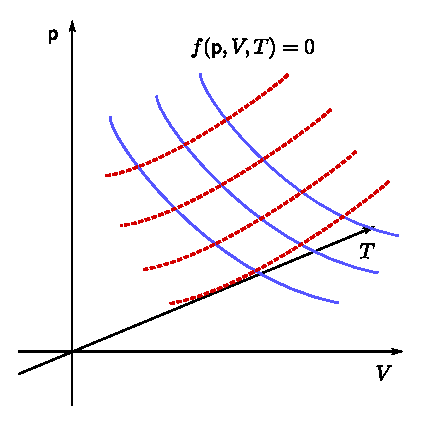
\includegraphics[width=\textwidth]{termo_2/termo_2_5}
            \newsubcap{$f(\pres,V,T)=0$ függvény, ami egy 3d-s felületet határoz meg a térben.}
            \label{fig:termo_2_5}
    \end{subfigure}\hfill
    \begin{subfigure}[]{0.45\textwidth}
            \centering
            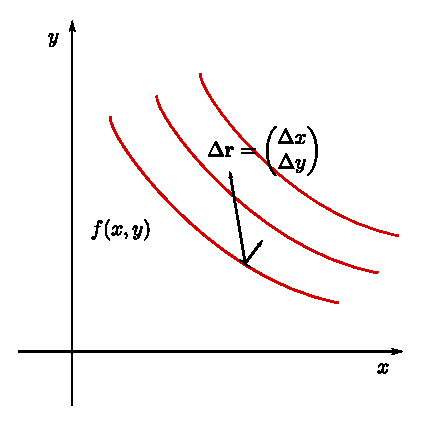
\includegraphics[width=\textwidth]{termo_2/termo_2_6}
            \newsubcap{Példa egy $f(x,y)$ kétváltozós függvény megváltozására.}
            \label{fig:termo_2_6}
    \end{subfigure}
\end{figure}
Ekkor az $f(x{+}\Delta x{,}y{+}\Delta y)$ kifejezést Taylor-sorba fejthetjük:
\begin{align}
    f(x{+}\Delta x,y{+}\Delta y)\approx f(x,y) + \bm\nabla f \Delta \bm r{+}\mathcal O(\Delta \bm r^2),\quad \tn{ahol}\quad \bm\nabla f \Delta \bm r = \pd fx\Delta x+\pd fy \Delta y.
\end{align}
A függvény megváltozása tehát elsőrendben:
\begin{align}
    \Delta f\approx \pd fx\Delta x+\pd fy \Delta y \follows \m df = \pd fx\bigg|_y\m d x+\pd fy\bigg|_x \m d y.
\end{align}
Ezutóbbit a függvény \emph{teljes deriváltjának} nevezzük. Alkalmazva ezt a $V(\pres,T)$ és $\pres(V,T)$ függvényekre kapjuk, hogy:
\begin{align}
    \m d V &= \pd V\pres\bigg|_T \m d\pres + \pd VT\bigg|_\pres \m dT \\
    \m d \pres &= \pd{\pres}{V}\bigg|_T\m dV + \pd{\pres}{T}\bigg|_V \m dT = \frac{1}{\pd{V}{\pres}\big|_T}\,\m d V - \frac{\pd{V}{T}\big|_\pres}{\pd{V}{\pres}\big|_T}\,\m d T,
\end{align}
ahol az utóbbi egyenlőségnél alkalmaztuk a hármasszabályt.
